\documentclass[9pt]{innovativeinnovation-cheatsheet}

\usepackage[utf8]{inputenc}
\usepackage[ngerman]{babel}

\usepackage{graphicx}

\usepackage{listings}
\usepackage{xcolor}

% Definiere eigene Farben
\definecolor{codegreen}{rgb}{0,0.6,0}
\definecolor{codegray}{rgb}{0.5,0.5,0.5}
\definecolor{codepurple}{rgb}{0.58,0,0.82}
\definecolor{backcolour}{rgb}{0.95,0.95,0.92}

% Listing-Stil für Shell-Scripts
\lstdefinestyle{mystyle}{
	backgroundcolor=\color{backcolour},   
	commentstyle=\color{codegreen},
	keywordstyle=\color{magenta},
	numberstyle=\tiny\color{codegray},
	stringstyle=\color{codepurple},
	basicstyle=\ttfamily\footnotesize,
	breakatwhitespace=false,         
	breaklines=true,                 
	captionpos=b,                    
	keepspaces=true,      
	numbers=none,            
	numbers=left,                    
	numbersep=5pt,                  
	showspaces=false,                
	showstringspaces=false,
	showtabs=false,                  
	tabsize=2
}

\lstset{style=mystyle}


\cheatsheettitle{Batch Processing - Cheat Sheet}


\begin{document}
    \begin{multicols*}{4}
	
	\cheatsheetsection{Einführung in Batch Processing} \ \\
	Batch Processing umfasst die Ausführung von Datenverarbeitungsaufgaben, die große Datenmengen in Batches sog. Stapeln bearbeiten. Diese Methode ist besonders geeignet für Prozesse, die nicht in Echtzeit ablaufen müssen, jedoch hochvolumige oder komplexe Datenmengen handhaben.
	
\textit{\textbf{Definition:}} \\
\textit{\textbf{Batch Processing bezieht sich auf das Sammeln von Daten in Gruppen oder Batches für die Verarbeitung. Ein typischer Batch-Prozess durchläuft mehrere Phasen – Sammeln, Verarbeiten, Ausgeben.}}
	
	\textbf{Beispiel für Batch-Verarbeitung:}
	\begin{itemize}
		\item Finanzbuchhaltung: Automatische Durchführung von Buchungen am Monats- oder Quartalsende.
		\item Telekommunikationsindustrie: Verarbeitung von Anrufdatensätzen (CDRs) zur Rechnungserstellung am Ende eines Abrechnungszyklus.
	\end{itemize}
	
	\textbf{Vorteile von Batch Processing:}
	\begin{itemize}
		\item \textbf{Effizienzsteigerung:} \\ Optimale Nutzung der Rechnerkapazitäten in Zeiten geringerer Nachfrage (z.B. nachts).
		\item \textbf{Skalierbarkeit:} \\ Einfache Skalierung der Datenverarbeitung mit zunehmender Datenmenge.
		\item \textbf{Kostenreduktion:} \\Minimierung der Kosten durch Automatisierung und Optimierung der Ressourcennutzung.
	\end{itemize}
	 
	\textbf{Anwendungsgebiete:}  \\
	Finanzbuchhaltung, ETL-Prozesse

\ \\
	
\cheatsheetsection{Einführung in die Linux/Unix Shell}

Die Shell in Unix/Linux-Systemen ist eine Befehlszeilen-Schnittstelle (CLI), die als mächtiges Werkzeug zur Verwaltung von Systemressourcen, zur Dateimanipulation, zur Prozesssteuerung und zur Automatisierung von Aufgaben genutzt wird.

\textbf{Grundlegende Shell-Befehle:} \ \\
Die Shell ermöglicht Interaktionen mit dem Betriebssystem über einfache Textbefehle. 

\begin{itemize}
	\item \textbf{ls:} Listet Dateien und Verzeichnisse auf.
	\item \textbf{cd:} Wechselt das Verzeichnis.
	\item \textbf{mkdir:} Erstellt ein Verzeichnis.
	\item \textbf{rm:} Entfernt Dateien oder Verzeichnisse.
	\item \textbf{cp:} Kopiert Dateien oder Verzeichnisse.
	\item \textbf{mv:} Verschiebt oder benennt Dateien oder Verzeichnisse um.
\end{itemize}

\textbf{Navigieren und Verwalten von Dateien:} \ \\
Effektives Navigieren und Verwalten von Dateisystemen ist eine grundlegende Fähigkeit für jeden Unix/Linux-Nutzer.

\begin{lstlisting}[language=bash, numbers=none]
cd Dokumente
ls
mkdir neues_verzeichnis
rm alte_datei.txt
\end{lstlisting}



\textbf{Bedeutung von Shell-Skripting:} \\
Shell-Skripting kombiniert mehrere Shell-Befehle in einer Datei zur automatischen Ausführung und erhöht die Effizienz bei wiederkehrenden Aufgaben.

\begin{lstlisting}[language=bash, numbers=none]
#!/bin/bash
echo "Starte die Aufgabe"
cp /pfad/zum/quellverzeichnis/* /pfad/zum/zielverzeichnis/
echo "Aufgabe abgeschlossen"
\end{lstlisting}

\cheatsheetsection{Batch Processing mit UNIX-Tools} \ \\ \\
\textbf{Einführung in UNIX-Tools für Batch-Processing:}
\begin{itemize}
	\item \textbf{Cron:} \\ Cron ist ein Planer, der automatisch Aufgaben zu festgelegten Zeiten ausführt. Du kannst es benutzen, um Dinge wie nächtliche Datensicherungen ohne dein Zutun durchzuführen.
	
	\item \textbf{Awk:}\\ Awk ist ein Tool zur Datenverarbeitung, das hilft, Textdateien Zeile für Zeile zu analysieren und zu bearbeiten, etwa um Berichte zu erstellen.
	
	\item \textbf{Sed:} \\ Sed ist ein Text-Editor, der direkt in der Kommandozeile funktioniert. Er ist nützlich, um schnelle Änderungen an Textdateien vorzunehmen, wie zum Beispiel das Ersetzen von Wörtern.
	
	\item \textbf{Grep:} \\ Grep ist ein Suchwerkzeug, das dir hilft, spezielle Zeilen in Textdateien zu finden, die bestimmte Wörter oder Phrasen enthalten.
\end{itemize}

\textbf{Automatisierung mit Cron:} \\
Cron hilft dir, Aufgaben zu einem festgelegten Zeitplan auszuführen, was nützlich ist, um wiederkehrende Jobs zu planen.

\textbf{Einfaches Beispiel für einen Cron-Job:} 
\begin{lstlisting}[language=bash, numbers=none]
	# Oeffnen der Crontab-Datei zur Bearbeitung:
	crontab -e
	
	# Ein Beispiel fuer einen Cron-Job, der taeglich um Mitternacht ausgefuehrt wird:
	0 0 * * * /pfad/zum/script.sh
\end{lstlisting}

\ \\ \\
\textbf{Datenverarbeitung mit Awk:} \\
Awk kann genutzt werden, um schnell Informationen aus Daten zu extrahieren.

\begin{lstlisting}[language=bash, numbers=none]
	# Hier ein einfacher Befehl, um die erste Spalte jeder Zeile in einer Datei auszugeben:
	awk '{print $1}' datei.txt
\end{lstlisting}

\textbf{Textmanipulation mit Sed:} \\
Mit Sed kannst du Text in Dateien einfach ändern.

\begin{lstlisting}[language=bash, numbers=none]
	# Ersetzt 'alt' mit 'neu' ueberall in 'datei.txt':
	sed 's/alt/neu/g' datei.txt
\end{lstlisting}

\textbf{Suchoperationen mit Grep:} \\
Grep hilft dir, schnell Zeilen zu finden, die bestimmte Muster enthalten.

\begin{lstlisting}[language=bash, numbers=none]
	# Zeigt Zeilen in 'datei.txt', die 'Muster' enthalten:
	grep 'Muster' datei.txt
\end{lstlisting}


\cheatsheetsection{MapReduce und verteilte Dateisysteme}

MapReduce ist ein Verfahren/Programmiermodell, das die Verarbeitung umfangreicher Datenmengen über ein Netzwerk verteilter Computer ermöglicht. Dieses Modell eignet sich hervorragend für Batch Processing, indem es komplexe Verarbeitungsoperationen in kleinere, unabhängige Einheiten unterteilt, die simultan auf verschiedenen Systemen ausgeführt werden können. Diese Methode ist besonders effektiv für Szenarien, in denen große Datenbestände in einem durchgehenden Prozess ohne direkte Interaktion des Endbenutzers bearbeitet werden.

\textbf{MapReduce Konzept} \\
MapReduce organisiert die Datenverarbeitung durch zwei sequentielle Phasen – \textbf{\textit{Map}} und \textbf{\textit{Reduce}}:
\begin{itemize}
	\item \textbf{Map-Phase:} Hier werden die Eingabedaten in Schlüssel-Wert-Paare umgewandelt. Jeder Eingabedatensatz wird unabhängig verarbeitet, was eine hohe Parallelisierung ermöglicht.
	\item \textbf{Reduce-Phase:} Nach der Map-Phase werden alle Zwischenschlüssel-Wert-Paare, die denselben Schlüssel haben, gruppiert und an die Reduce-Funktion weitergeleitet, die sie zu einem einzelnen Ausgabewert zusammenfasst.
\end{itemize}

\textbf{Einfaches Python-Beispiel für MapReduce:} \\
In diesem Beispiel wird die Häufigkeit jedes Wortes in einem Textdokument gezählt:

\begin{lstlisting}[language=python, numbers=none]
from mrjob.job import MRJob
	
class MRWordFrequencyCount(MRJob):
	def mapper(self, _, line):
		# Split the line into words
		words = line.split()
		# Emit each word with a count of 1
		for word in words:
			yield word, 1
	
	def reducer(self, key, values):
		# Sum all the counts for each word
		total = sum(values)
		yield key, total
	
if __name__ == '__main__':
	MRWordFrequencyCount.run()
\end{lstlisting}



\cheatsheetsection{Hadoop Distributed File System (HDFS)}


Das Hadoop Distributed File System (HDFS) ist ein System, das entwickelt wurde, um sehr große Mengen von Daten über viele Computer in einem Netzwerk zu verteilen und zu speichern. Es ist ein wesentlicher Bestandteil von Hadoop, einer Software, die große Datenmengen verarbeiten kann.

\textbf{Was macht HDFS besonders?} \\
- \textbf{Skalierbarkeit:} HDFS kann sehr groß werden, indem es mehr Computer in das Netzwerk einbindet, sodass es mit wachsenden Datenmengen mithalten kann. \\
- \textbf{Fehlertoleranz:} Es kopiert Daten automatisch auf mehrere Computer, so dass keine Daten verloren gehen, selbst wenn einige Computer ausfallen. \\
- \textbf{Hohe Verfügbarkeit:} Die Daten sind jederzeit verfügbar, auch wenn Teile des Systems ausfallen, dank der Kopien auf verschiedenen Computern. \\
- \textbf{Kosteneffizienz:} Es kann auf normaler, nicht spezialisierter Hardware betrieben werden, was Kosten spart.

\textbf{Wie funktioniert HDFS?} \\
- \textbf{NameNode:} Dies ist der Hauptcomputer, der überwacht, wo alle Datenstücke im Netzwerk gespeichert sind. \\
- \textbf{DataNode:} Diese Computer speichern und verwalten die eigentlichen Daten. Sie nehmen Anweisungen vom NameNode entgegen, um Daten zu lesen, zu schreiben und zu löschen.

\textbf{Zusammenarbeit mit MapReduce:} \\
HDFS arbeitet eng mit MapReduce zusammen, einem weiteren Tool von Hadoop, das dazu dient, die Daten zu analysieren und aufzubereiten. Zusammen ermöglichen sie es, komplexe Analysen mit großen Datenmengen effizient durchzuführen.

\textbf{Anwendungen von HDFS:} \\
HDFS wird in vielen verschiedenen Bereichen eingesetzt, darunter in der Web-Indexierung, in sozialen Netzwerken und in der Datenanalyse, wo große Mengen von Daten gespeichert und schnell verarbeitet werden müssen.


\cheatsheetsection{Prozessveranschaulichung}  \\ \\
Das folgende Diagramm veranschaulicht den typischen Ablauf eines MapReduce-Jobs innerhalb eines Hadoop Distributed File System (HDFS). Es zeigt die parallele Natur der Map- und Reduce-Aufgaben sowie den Datenfluss zwischen diesen Komponenten.
\begin{center}
	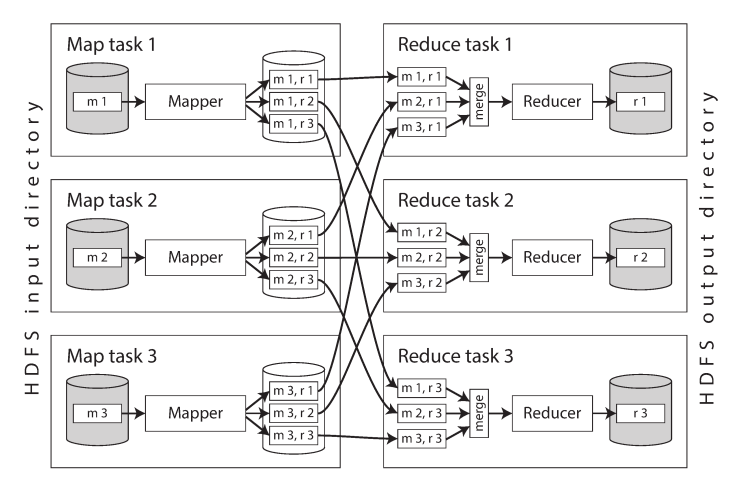
\includegraphics[width=0.99\linewidth]{MapReduce}
\end{center}


\textbf{Beschreibung des Diagramms:}
\begin{itemize}
\item \textbf{Map Tasks:} Jede Map Task verarbeitet einen Teil der Eingabedaten unabhängig von den anderen. Beispielsweise liest Map Task 1 Daten aus dem ersten Block des HDFS-Inputverzeichnisses.
\item \textbf{Reducer Tasks:} Jede Reduce Task sammelt und verarbeitet die Zwischenergebnisse, die von den Map Tasks erzeugt wurden, um das Endresultat zu erstellen. Reducer 1 beispielsweise aggregiert Ergebnisse, die den gleichen Schlüssel (z.B. r1) teilen.
\end{itemize}


\cheatsheetsection{Nachteile von Batch Processing / MapReduce und HDFS} \\ \\
\textbf{Nachteile von Batch Processing:} \\
Batch Processing, obwohl effizient für große Datenmengen, hat einige Einschränkungen:
\begin{itemize}
	\item \textbf{Zeitverzögerungen:} Da Prozesse in Batches ausgeführt werden, kann es zu Verzögerungen kommen, bevor Ergebnisse verfügbar sind.
	\item \textbf{Ressourcenintensiv:} Große Datenmengen erfordern signifikante Rechenressourcen, was insbesondere bei begrenzter Infrastruktur zu Problemen führen kann.
	\item \textbf{Komplexität:} Die Verwaltung und Überwachung von Batch Jobs kann komplex sein, insbesondere wenn Fehlerbehandlung und Wiederanlauf von Prozessen notwendig werden.
\end{itemize}

\textbf{Nachteile von MapReduce und HDFS:}
\begin{itemize}
	\item \textbf{Skalierbarkeitsgrenzen:} Obwohl Hadoop hervorragend skalierbar ist, kann die Leistung bei extrem großen Datenmengen oder sehr schnellen Datenströmen nachlassen.
	\item \textbf{Komplexität der Verwaltung:} HDFS erfordert eine aufmerksame Verwaltung der DataNodes und NameNodes, was die Systemkomplexität erhöht.
	\item \textbf{Langsamere Verarbeitung:} MapReduce ist nicht optimal für Prozesse, die Echtzeitanalysen benötigen, da die Verarbeitung von Daten in Batches erfolgt.
\end{itemize}


\cheatsheetsection{Batch Processing vs. Stream Processing}

\begin{center}
	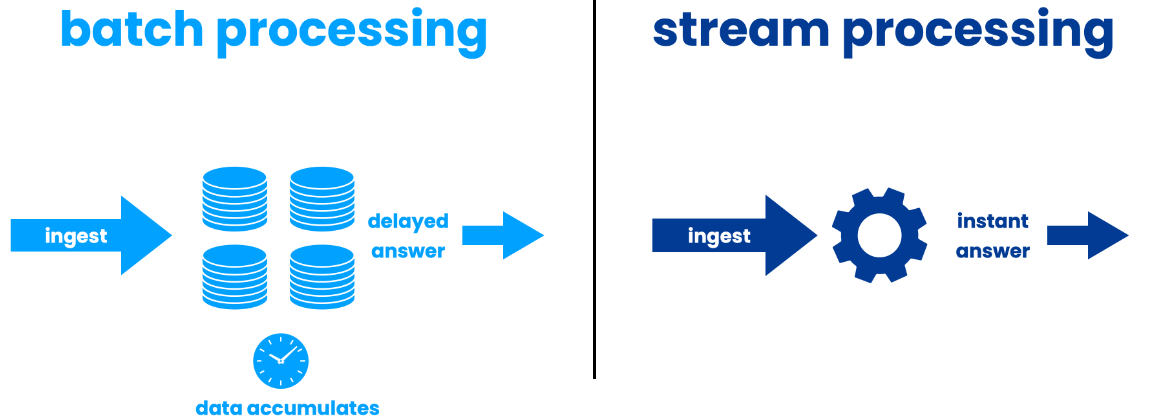
\includegraphics[width=0.99\linewidth]{batch_stream}
\end{center}










	
\end{multicols*}
\end{document}
